\chapter{Phân tích yêu cầu hệ thống}

\section{Giới thiệu chương}

Chương này trình bày quá trình phân tích yêu cầu đối với hệ thống AIConnect. Nội dung bao gồm mô tả bài toán, xác định các tác nhân tham gia, phân tích yêu cầu chức năng và phi chức năng, xây dựng các mô hình UML như Use Case Diagram, Activity Diagram và Sequence Diagram nhằm mô tả nghiệp vụ và hành vi của hệ thống. Kết quả của chương là cơ sở cho việc thiết kế cơ sở dữ liệu, kiến trúc hệ thống và triển khai ứng dụng trong các chương tiếp theo.

\section{Mô tả bài toán}

\subsection{Bối cảnh}

Trong thời đại chuyển đổi số, trí tuệ nhân tạo (AI) đang được ứng dụng rộng rãi trong nhiều lĩnh vực như chăm sóc khách hàng, phân tích dữ liệu, tự động hóa quy trình nghiệp vụ và marketing. Việc ứng dụng AI giúp doanh nghiệp nâng cao hiệu quả hoạt động, giảm chi phí vận hành và tăng khả năng cạnh tranh.

Tuy nhiên, phần lớn doanh nghiệp hiện nay chưa sở hữu đội ngũ AI chuyên nghiệp. Việc tìm kiếm chuyên gia phù hợp để triển khai các giải pháp AI còn gặp nhiều khó khăn về thời gian, chi phí và độ tin cậy.

\subsection{Thực trạng}

Các doanh nghiệp thường tìm kiếm chuyên gia AI thông qua các nền tảng tuyển dụng hoặc mạng xã hội. Cách thức này tồn tại nhiều hạn chế:

\begin{itemize}
    \item Khó đánh giá năng lực thực tế của chuyên gia.
    \item Tốn thời gian sàng lọc hồ sơ.
    \item Thiếu công cụ quản lý dự án chuyên nghiệp.
    \item Khó kiểm soát chất lượng dịch vụ.
    \item Không có cơ chế gợi ý chuyên gia phù hợp.
\end{itemize}

Trong khi đó, các chuyên gia AI cũng gặp khó khăn trong việc tiếp cận khách hàng tiềm năng và tìm kiếm các dự án phù hợp với chuyên môn của mình.

\subsection{Giải pháp đề xuất}

Đề tài đề xuất xây dựng hệ thống AIConnect – nền tảng kết nối doanh nghiệp với các chuyên gia AI.

Hệ thống cho phép doanh nghiệp đăng tải nhu cầu triển khai AI, tìm kiếm chuyên gia phù hợp và quản lý quá trình hợp tác. Đồng thời, chuyên gia AI có thể xây dựng hồ sơ năng lực, tìm kiếm dự án và gửi đề xuất hợp tác đến doanh nghiệp.

Ngoài ra, hệ thống tích hợp chức năng AI Matching nhằm tự động đề xuất các chuyên gia phù hợp dựa trên kỹ năng, kinh nghiệm và lịch sử dự án.

\section{Xác định tác nhân hệ thống}

Hệ thống AIConnect có ba tác nhân chính.

\subsection{Doanh nghiệp (Enterprise)}

Doanh nghiệp là đối tượng sử dụng hệ thống để tìm kiếm chuyên gia AI phục vụ cho nhu cầu tự động hóa và chuyển đổi số.

Các chức năng chính:

\begin{itemize}
    \item Đăng ký, đăng nhập.
    \item Đăng dự án AI.
    \item Tìm kiếm chuyên gia.
    \item Thuê chuyên gia.
    \item Thanh toán.
    \item Đánh giá chất lượng dịch vụ.
\end{itemize}

\subsection{Chuyên gia AI (Expert)}

Chuyên gia AI là cá nhân hoặc tổ chức cung cấp dịch vụ tư vấn và triển khai giải pháp AI.

Các chức năng chính:

\begin{itemize}
    \item Tạo hồ sơ năng lực.
    \item Ứng tuyển dự án.
    \item Quản lý công việc.
    \item Trao đổi với doanh nghiệp.
    \item Nhận thanh toán.
\end{itemize}

\subsection{Quản trị viên (Admin)}

Quản trị viên chịu trách nhiệm vận hành hệ thống.

Các chức năng chính:

\begin{itemize}
    \item Quản lý người dùng.
    \item Kiểm duyệt nội dung.
    \item Quản lý giao dịch.
    \item Thống kê hoạt động hệ thống.
\end{itemize}

\section{Danh sách Use Case}

\begin{table}[H]
\centering
\caption{Danh sách Use Case của hệ thống}
\label{tab:usecase}
\begin{tabular}{|c|p{5cm}|c|}
\hline
\textbf{Mã} & \textbf{Tên Use Case} & \textbf{Tác nhân} \\
\hline
UC01 & Đăng ký tài khoản & Tất cả \\
\hline
UC02 & Đăng nhập & Tất cả \\
\hline
UC03 & Đăng dự án AI & Doanh nghiệp \\
\hline
UC04 & Tìm kiếm chuyên gia & Doanh nghiệp \\
\hline
UC05 & AI Matching chuyên gia & Doanh nghiệp \\
\hline
UC06 & Tạo hồ sơ chuyên gia & Chuyên gia \\
\hline
UC07 & Ứng tuyển dự án & Chuyên gia \\
\hline
UC08 & Ký hợp đồng & Doanh nghiệp, Chuyên gia \\
\hline
UC09 & Quản lý tiến độ & Doanh nghiệp, Chuyên gia \\
\hline
UC10 & Chat trực tuyến & Doanh nghiệp, Chuyên gia \\
\hline
UC11 & Thanh toán & Doanh nghiệp \\
\hline
UC12 & Đánh giá dự án & Doanh nghiệp, Chuyên gia \\
\hline
UC13 & Quản lý người dùng & Admin \\
\hline
UC14 & Kiểm duyệt nội dung & Admin \\
\hline
UC15 & Xem thống kê & Admin \\
\hline
\end{tabular}
\end{table}

Bảng \ref{tab:usecase} mô tả toàn bộ các chức năng chính của hệ thống AIConnect.

\section{Biểu đồ Use Case}

\begin{figure}[H]
\centering
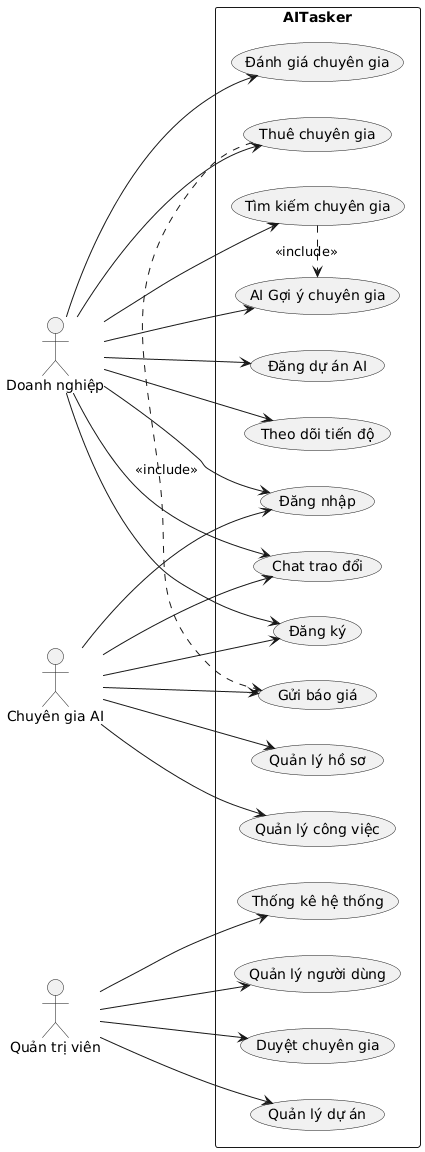
\includegraphics[width=0.85\textwidth]{figures/imagesusecase.png}
\caption{Biểu đồ Use Case của hệ thống AIConnect}
\label{fig:usecase}
\end{figure}

\section{Biểu đồ Activity}

\subsection{Activity Diagram chức năng đăng dự án}

\begin{figure}[H]
\centering
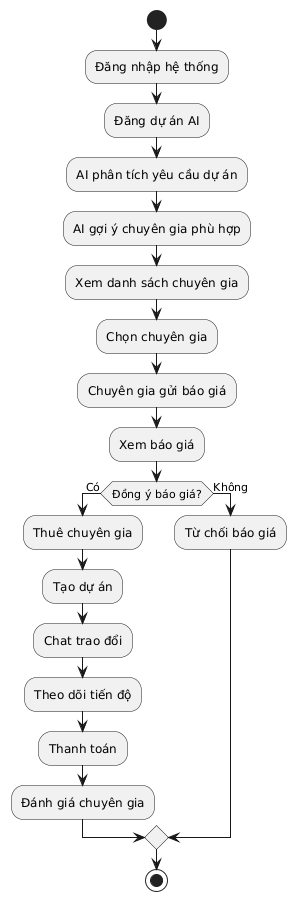
\includegraphics[width=0.75\textwidth]{figures/figuresactivity-project.png}
\caption{Activity Diagram chức năng đăng dự án}
\label{fig:activity-project}
\end{figure}

\subsection{Activity Diagram chức năng Matching chuyên gia}

\begin{figure}[H]
\centering
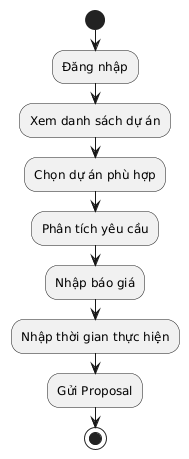
\includegraphics[width=0.75\textwidth]{figures/activity2.png}
\caption{Activity Diagram chức năng Matching chuyên gia}
\label{fig:activity-matching}
\end{figure}

\section{Biểu đồ Sequence}

\subsection{Sequence Diagram chức năng đăng dự án}

\begin{figure}[H]
\centering
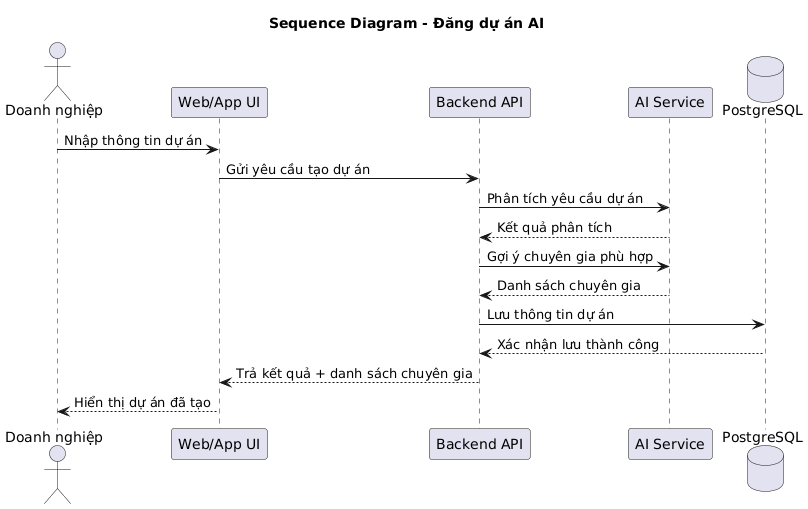
\includegraphics[width=0.85\textwidth]{figures/sequence1.png}
\caption{Sequence Diagram chức năng đăng dự án}
\label{fig:sequence-project}
\end{figure}

\subsection{Sequence Diagram chức năng ứng tuyển dự án (Gửi báo giá)}

\begin{figure}[H]
\centering
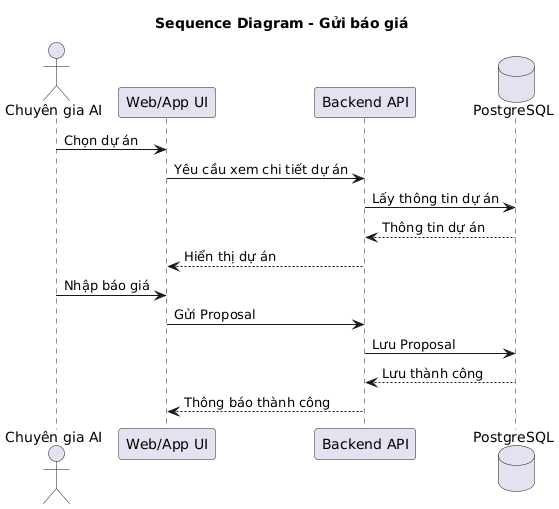
\includegraphics[width=0.85\textwidth]{figures/sequence2.png}
\caption{Sequence Diagram chức năng ứng tuyển dự án (Gửi báo giá)}
\label{fig:sequence-proposal}
\end{figure}

\subsection{Sequence Diagram chức năng thuê chuyên gia}

\begin{figure}[H]
\centering
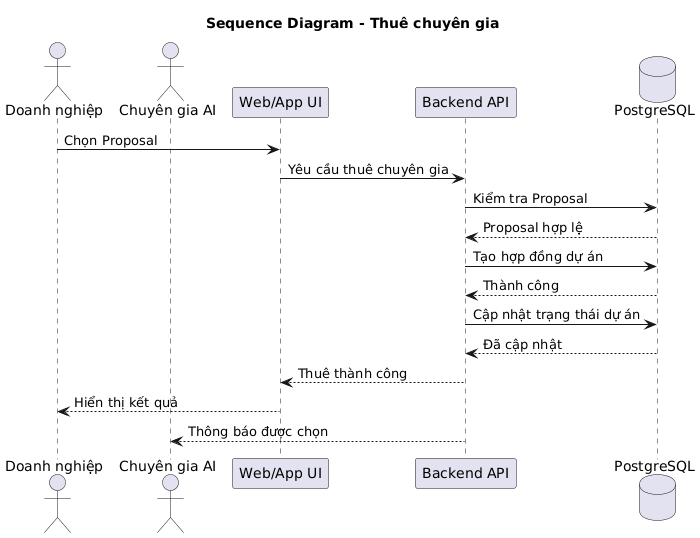
\includegraphics[width=0.85\textwidth]{figures/sequence3.png}
\caption{Sequence Diagram chức năng thuê chuyên gia}
\label{fig:sequence-hire}
\end{figure}

\section{Biểu đồ lớp (Class Diagram)}

Biểu đồ lớp mô tả cấu trúc tĩnh của hệ thống AIConnect, bao gồm các lớp dữ liệu chính, thuộc tính, phương thức và mối quan hệ giữa các lớp trong hệ thống.

Các lớp trung tâm bao gồm:

\begin{itemize}
    \item User
    \item Enterprise
    \item Expert
    \item Project
    \item Proposal
    \item Contract
    \item Payment
    \item Message
    \item Review
    \item Admin
\end{itemize}

Thông qua biểu đồ lớp có thể thấy cách tổ chức dữ liệu và luồng tương tác giữa các thành phần nghiệp vụ của hệ thống.

\begin{figure}[H]
\centering
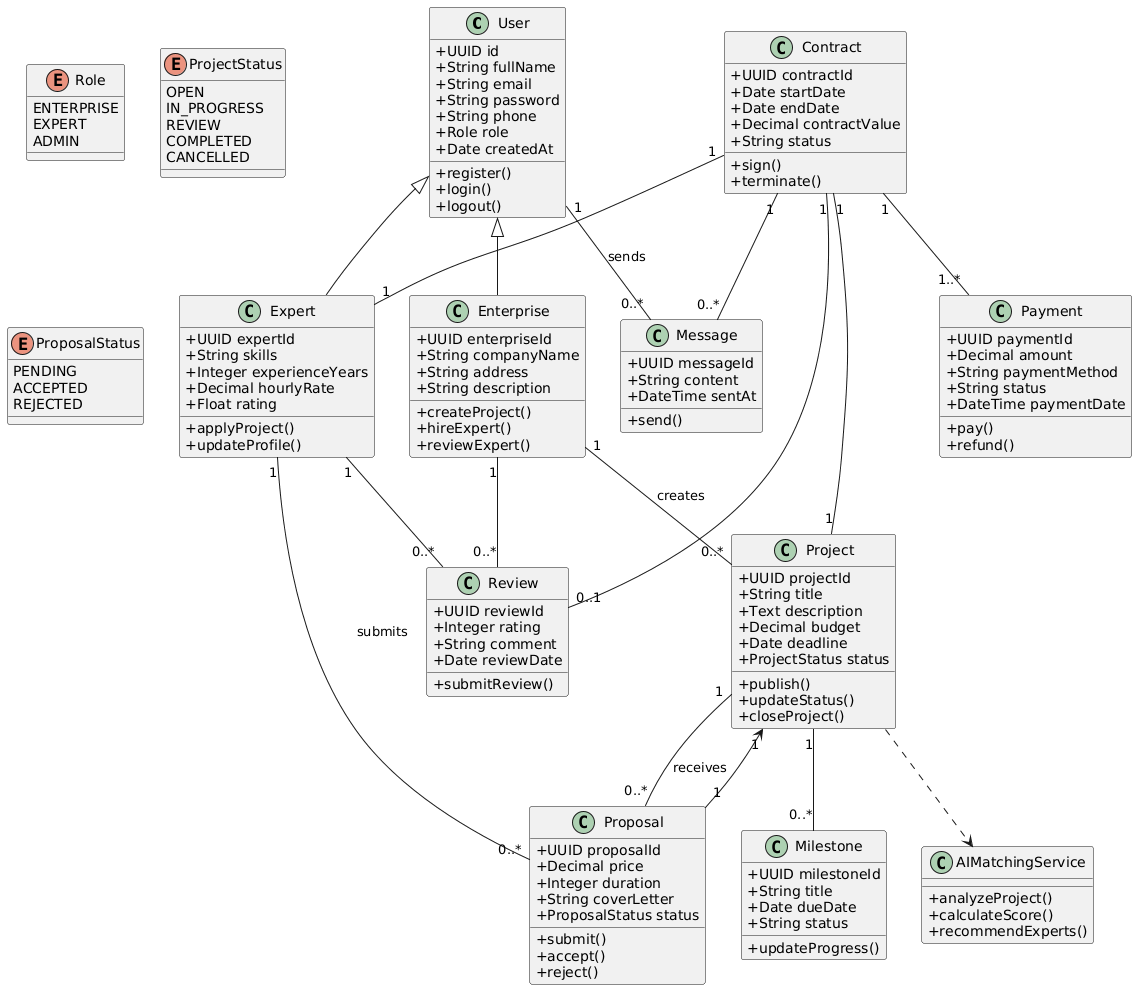
\includegraphics[width=0.9\textwidth]{figures/Class.png}
\caption{Class Diagram của hệ thống AIConnect}
\label{fig:class}
\end{figure}

\section{Yêu cầu phi chức năng}

\subsection{Hiệu năng}

\begin{itemize}
    \item Thời gian phản hồi trung bình dưới 2 giây.
    \item Hỗ trợ tối thiểu 500 người dùng đồng thời.
\end{itemize}

\subsection{Bảo mật}

\begin{itemize}
    \item Sử dụng HTTPS.
    \item Xác thực JWT.
    \item Mã hóa mật khẩu bằng BCrypt.
    \item Phân quyền theo vai trò người dùng.
\end{itemize}

\subsection{Khả năng mở rộng}

\begin{itemize}
    \item Hỗ trợ mở rộng theo chiều ngang.
    \item Dễ dàng tích hợp thêm các dịch vụ AI mới.
\end{itemize}

\subsection{Tính sẵn sàng}

\begin{itemize}
    \item Hoạt động 24/7.
    \item Đảm bảo thời gian hoạt động tối thiểu 99.5\%.
\end{itemize}

\subsection{Khả năng sử dụng}

\begin{itemize}
    \item Giao diện thân thiện.
    \item Dễ dàng sử dụng đối với người mới.
\end{itemize}

\section{Kết luận chương}

Chương này đã trình bày quá trình phân tích yêu cầu của hệ thống AIConnect, bao gồm mô tả bài toán, xác định các tác nhân tham gia, phân tích các yêu cầu chức năng và phi chức năng, đồng thời xây dựng các mô hình UML để mô tả hoạt động của hệ thống. Đây là cơ sở quan trọng để thực hiện thiết kế hệ thống và xây dựng cơ sở dữ liệu ở chương tiếp theo.